\section{Experiments and Results}

\begin{frame}{Experiments}
    Four types of experiments were conducted, each involving a single pass through 1000 problems due to cost constraints.

    \begin{enumerate}
        \item \textbf{Full System:} The CoT-SelfEvolve model was evaluated alongside six different Language Learning Models (LLMs), including GPT-3.5-turbo, GPT-4, Claude 2.1, Claude 3, Mistral Large, and Mistral 8x7B.

        \item \textbf{Auto-CoT Generators:} The functionality of Auto-CoT generators was toggled on and off to examine their impact on the performance of CoT-SelfEvolve.

        \item \textbf{Large LLM as Teacher:} A large LLM, such as GPT-4, was used for CoT prompt generation, while GPT-3.5-turbo was used for code generation.

        \item \textbf{Auto-CoT with Code LLM:} The initial Auto-CoT prompt generator was evaluated using the specialized code LLM (Llama 3 70B).
    \end{enumerate}
\end{frame}

\begin{frame}{Result: Full System}
    The CoT-SelfEvolve model, employing GPT-4 as the base LLM, outperformed the original SelfEvolve model in handling Pytorch, Sklearn, and Matplotlib questions, demonstrating a clear superiority.

    \begin{table}[H]
        \caption*{$\text{Pass@5}$ results on the DS-1000 dataset. (\%)}
        \resizebox{\textwidth}{!}{%
            \begin{tabular}{|l|l|c|c|c|c|c|c|c|c|}
                \hline
                                                & LLM           & \multicolumn{1}{l|}{Scipy} & \multicolumn{1}{l|}{PyTorch} & \multicolumn{1}{l|}{Sklearn} & \multicolumn{1}{l|}{Matplotlib} & \multicolumn{1}{l|}{Pandas} & \multicolumn{1}{l|}{Numpy} & \multicolumn{1}{l|}{TensorFlow} & \multicolumn{1}{l|}{Overall} \\ \hline
                \multirow{2}{*}{SelfEvolve}     & GPT-3.5       & 52.83                      & 64.71                        & 73.04                        & 78.06                           &                             &                            &                                 & \multicolumn{1}{l|}{}        \\ \cline{2-10}
                                                & GPT-4         & \textbf{58.49}             & 70.59                        & 70.43                        & 84.52                           &                             &                            &                                 & \multicolumn{1}{l|}{}        \\ \hline
                \multirow{6}{*}{CoT-SelfEvolve} & GPT-3.5       & 32.08                      & 72.06                        & 66.09                        & 32.26                           & 29.55                       & 17.73                      & 46.67                           & 35.5                         \\ \cline{2-10}
                                                & GPT-4         & 53.77                      & \textbf{89.71}               & \textbf{97.39}               & \textbf{85.16}                  & \textbf{92.78}              & \textbf{76.36}             & \textbf{84.44}                  & \textbf{83.8}                \\ \cline{2-10}
                                                & Claude 2.1    & 47.17                      & 83.82                        & 85.22                        & 83.23                           & 65.64                       & 61.82                      & 57.78                           & 68.7                         \\ \cline{2-10}
                                                & Claude 3      & 44.34                      & 76.47                        & 73.91                        & 85.81                           & 43.64                       & 31.36                      & 53.33                           & 53.7                         \\ \cline{2-10}
                                                & Mistral Large & 45.28                      & 80.88                        & 78.26                        & 52.26                           & 68.04                       & 43.64                      & 53.33                           & 59.2                         \\ \cline{2-10}
                                                & Mistral 8x7B  & 30.19                      & 57.35                        & 56.52                        & 69.68                           & 38.49                       & 35.91                      & 44.44                           & 45.5                         \\ \hline
            \end{tabular}%
        }
    \end{table}
\end{frame}

\begin{frame}{Result: Auto-CoT Generators}
    The performance enhancement brought about by the Auto-CoT prompt generators is evident when compared to the non-CoT prompt version, with a relative gain of \textbf{16.39\%}. This finding highlights the significance of Auto-CoT prompt generators in augmenting the efficacy of the CoT-SelfEvolve model.

    \begin{table}[H]
        \caption*{$\text{Pass@5}$ results on the DS-1000 dataset w or w/o CoT prompts. (\%)}
        \resizebox{\textwidth}{!}{%
            \begin{tabular}{|c|c|c|c|c|c|c|c|c|c|}
                \hline
                Auto-CoT 1 & Auto-CoT 2 & Scipy & PyTorch & Sklearn & Matplotlib & Pandas & Numpy & TensorFlow & Overall \\ \hline
                off        & off        & 33.02 & 64.71   & 59.13   & 26.45      & 23.02  & 14.09 & 42.22      & 30.5    \\ \hline
                on         & off        & 28.3  & 75      & 63.48   & 29.68      & 29.21  & 17.27 & 51.11      & 34.6    \\ \hline
                on         & on         & 32.08 & 72.06   & 66.09   & 32.26      & 29.55  & 17.73 & 46.67      & 35.5    \\ \hline
                off        & on         & 23.58 & 66.18   & 53.91   & 29.68      & 30.24  & 18.18 & 42.22      & 32.4    \\ \hline
            \end{tabular}%
        }
    \end{table}
\end{frame}

\begin{frame}{Result: Large LLM as Teacher}
    The data clearly shows that leveraging a larger LLM to steer the code generation process can significantly enhance the model's performance, as evidenced by a relative gain of \textbf{11.26\%}.

    \begin{table}[H]
        \caption*{$\text{Pass@5}$ results on the DS-1000 dataset with different LLM stacks. (\%)}
        \centering
        \resizebox{\columnwidth}{!}{%
            \begin{tabular}{|c|c|c|c|c|c|c|c|c|c|}
                \hline
                Auto-CoT LLM & Code LLM & Scipy & PyTorch & Sklearn & Matplotlib & Pandas & Numpy & TensorFlow & Overall \\ \hline
                GPT-3.5 & GPT-3.5  & 32.08 & 72.06   & 66.09   & 32.26      & 29.55  & 17.73 & 46.67      & 35.5    \\ \hline
                GPT-4   & GPT-3.5  & 37.74 & 83.82   & 73.04   & 35.48      & 31.62  & 19.55 & 53.33      & 39.5    \\ \hline
            \end{tabular}%
        }
    \end{table}
\end{frame}

\begin{frame}{Result: Auto-CoT with Code LLM}
    \begin{figure}[H]
        \centering
        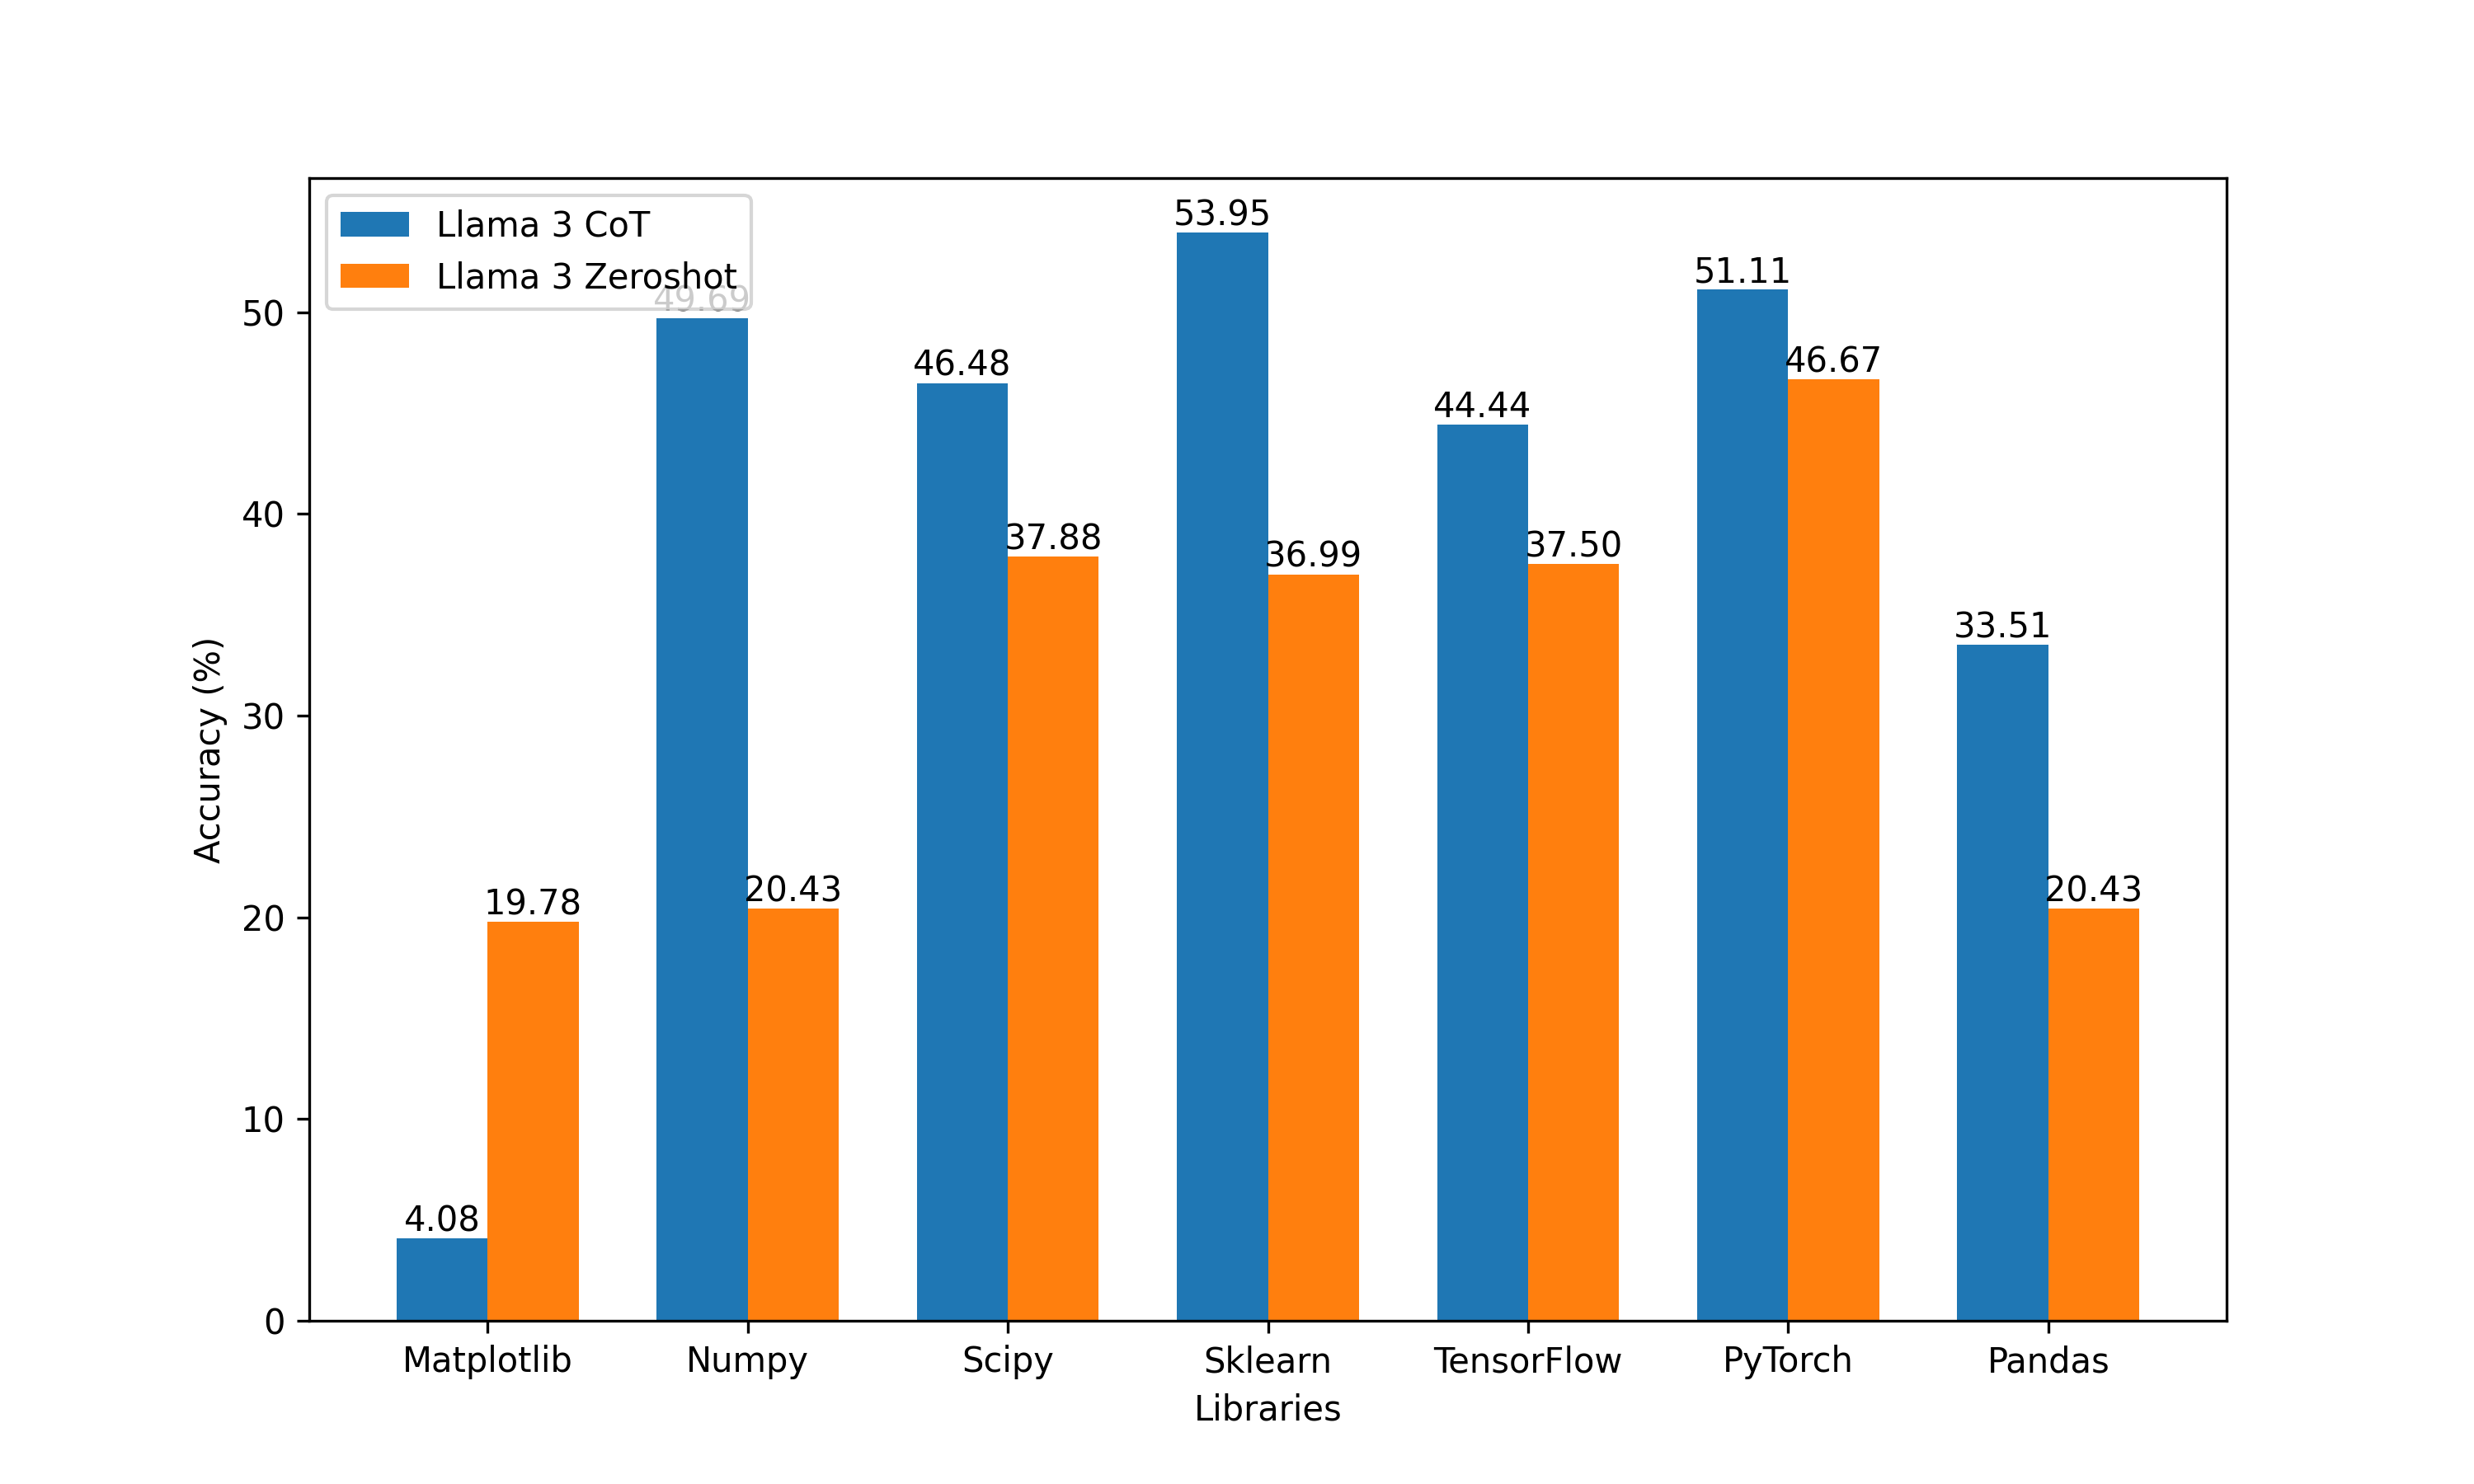
\includegraphics[width=\columnwidth]{img/code_llm}
        \caption*{Comparison of Llama 3 CoT and Zeroshot (without self-correction).}
    \end{figure}
\end{frame}
